First of all it is necessary to classify the different recipients of the analysed messages. For this purpose, all the contacts (a total of 337 different e-mail addresses) have been divided into twelve categories depending on their relationship with the analysed user. These categories are: friend, acquaintance, company (in this category are grouped all the company contacts with which the user has had a relationship to contract their service), university, boss, colleague, professor, relative, stranger, university position, casting (the people with which the user was in touch in order to manage a theatre casting belong to this relationship type) and company recruiting (where are classified the e-mail addresses that the user contacted to be a candidate in a recruiting process).

Our style markers were applied to each message, so it is necessary to categorise the different e-mails. With this in mind, we will determine the category of the message depending on its recipient(s). Classifying e-mails destined for a single e-mail account is a trivial problem (its category will be the one assigned to the message's recipient). We can also directly classify those messages whose recipients all belong to the same category. E-mails that have several receivers from different categories are automatically classified when they have only one addressee in the recipients field \textit{To} (they are grouped in that contact's category), which represents the main recipient(s) of the message, while the \textit{Cc} (Carbon Copy) and \textit{Bcc} (Blind Carbon Copy) fields have the purpose of keeping the addressees in there informed. Otherwise, we classify it one by one (there were only 14 messages out of 921 that we had to review) depending on the type of relationship we think indicates the wording of the message.

After this classification process, we obtained the distribution of relationship categories that we can see in Figure \ref{fig:distr}. As we can observe, we have not equal distributed classes and this will represent a problem in our data analysis. Indeed, the biggest class (the professor class) represents approximately $39.41$\% of the total, while the second one (university position) in size is the $13.25$\%. And, of course, both categories are far from the smallest class (acquaintance) which only represents approximately $0.33$\%. Despite this unbalanced distribution between the different categories, we are going to analyse this data set and obtain conclusions in order to detect the most significant features for differentiating the writing style based on the recipient of the e-mail. We have to take into account that the conclusions will be closely linked to the data obtained given the small sample size.

\begin{figure}
	\centering%
	\centerline{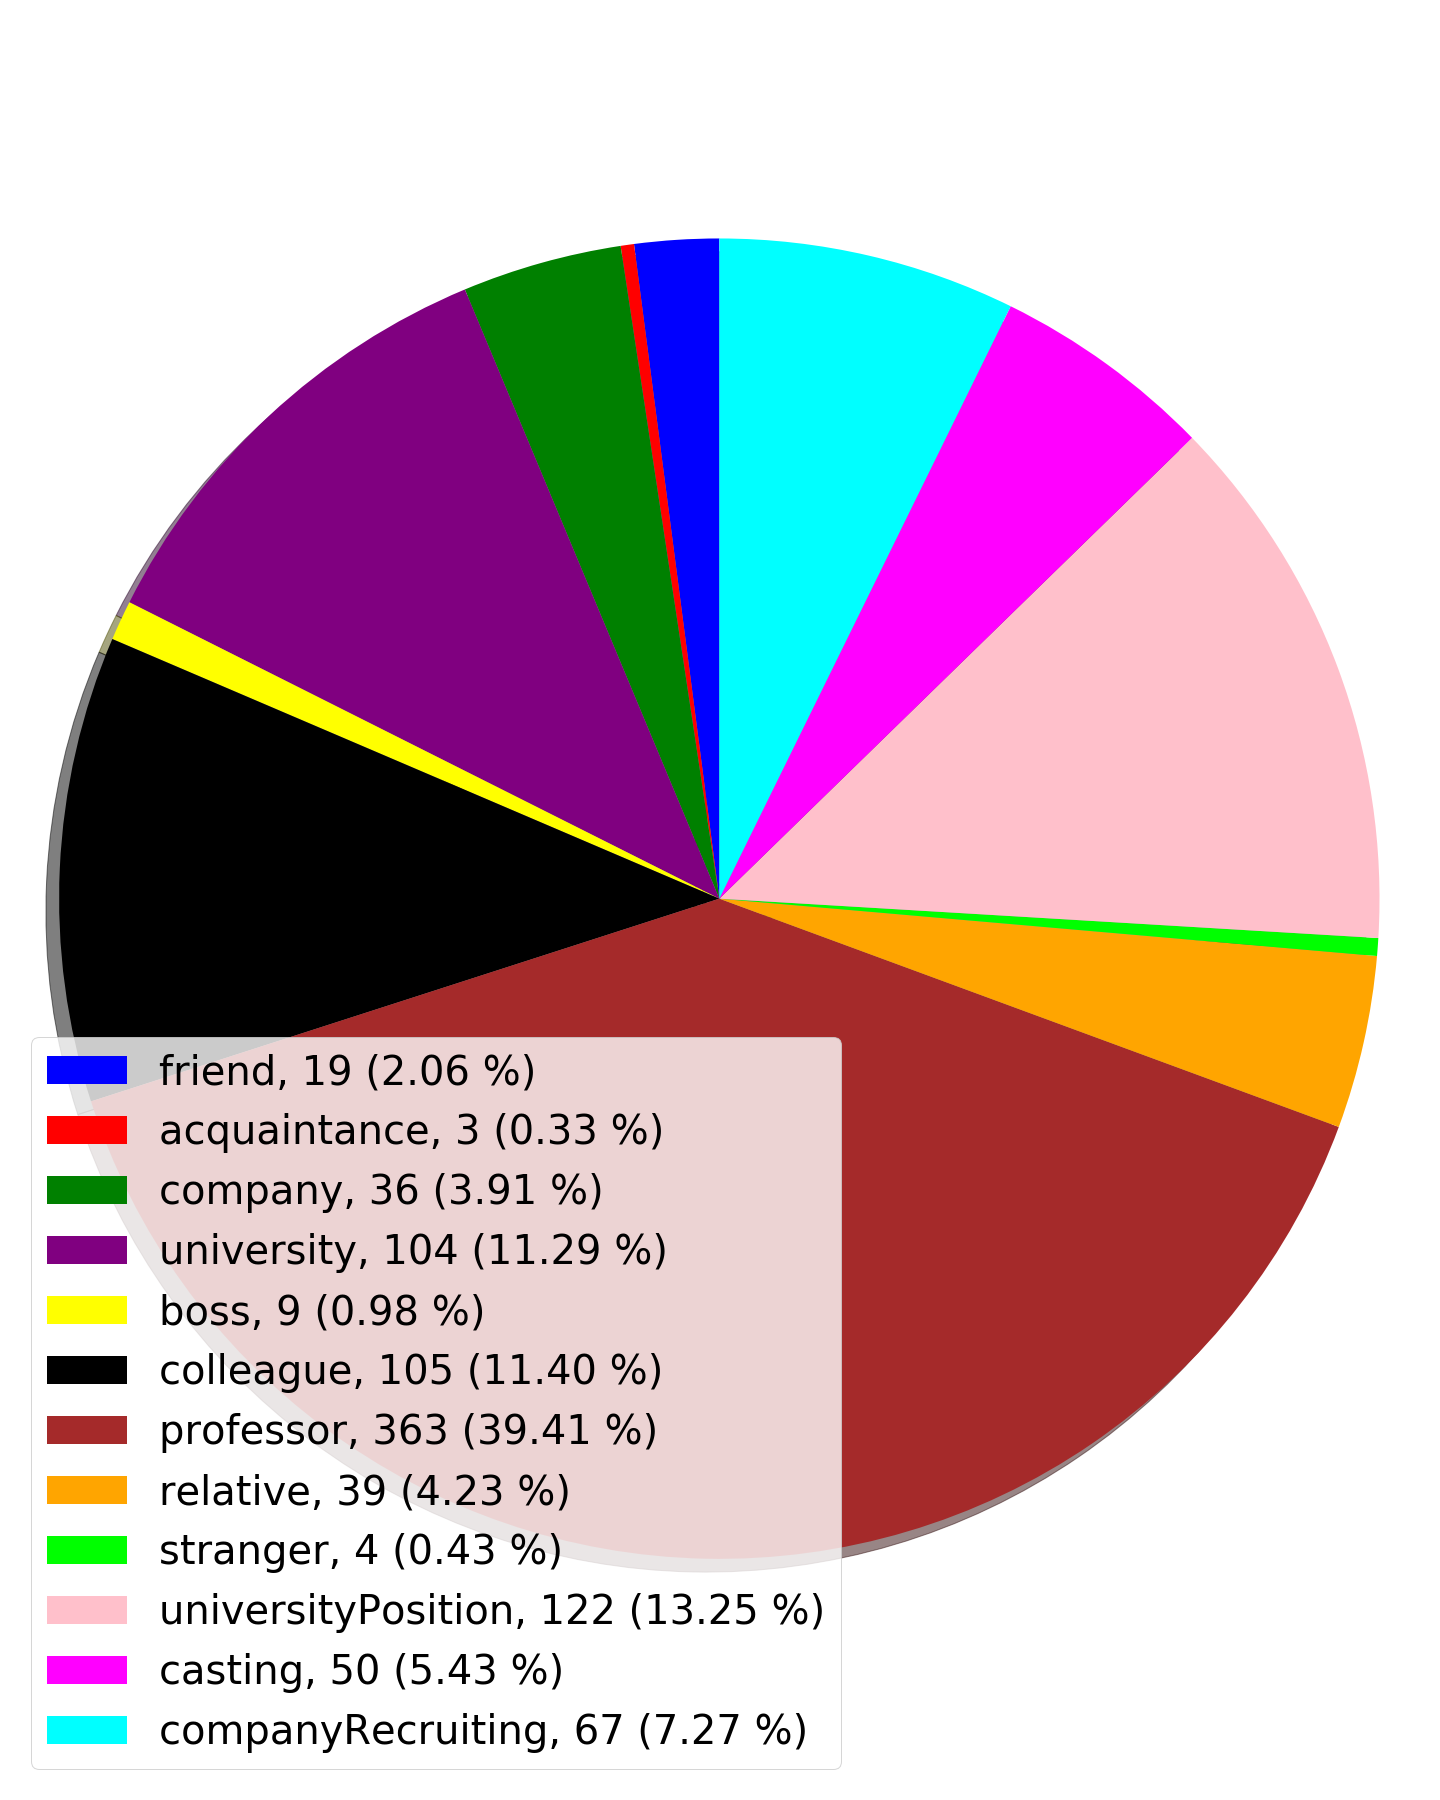
\includegraphics[width=0.5\textwidth]{Imagenes/Bitmap/classdistributionpie.png}}%
	\caption{Distribution of relationship categories}%
	\label{fig:distr}
\end{figure}

Once all e-mails are classified in our twelve categories, we have to choose which style features we are going to analyse. At first glance, there are features of each message (the attributes of the \textit{Metrics} class, which can be looked up in Section \ref{section:measmod}) from which we are not be able to extract significant numerical information, such as the sender of the e-mails (which is the same for all of them), the subject and the identifier of the thread they belong to (called \textit{threadId}). Besides, as the distribution of the different categories is too unbalanced, we risk losing underrepresented classes if a time-related weight is applied over the several metrics. For this reason, we decide not to take the date into account for our analysis.

\begin{figure}[p]
	\centering%
	\centerline{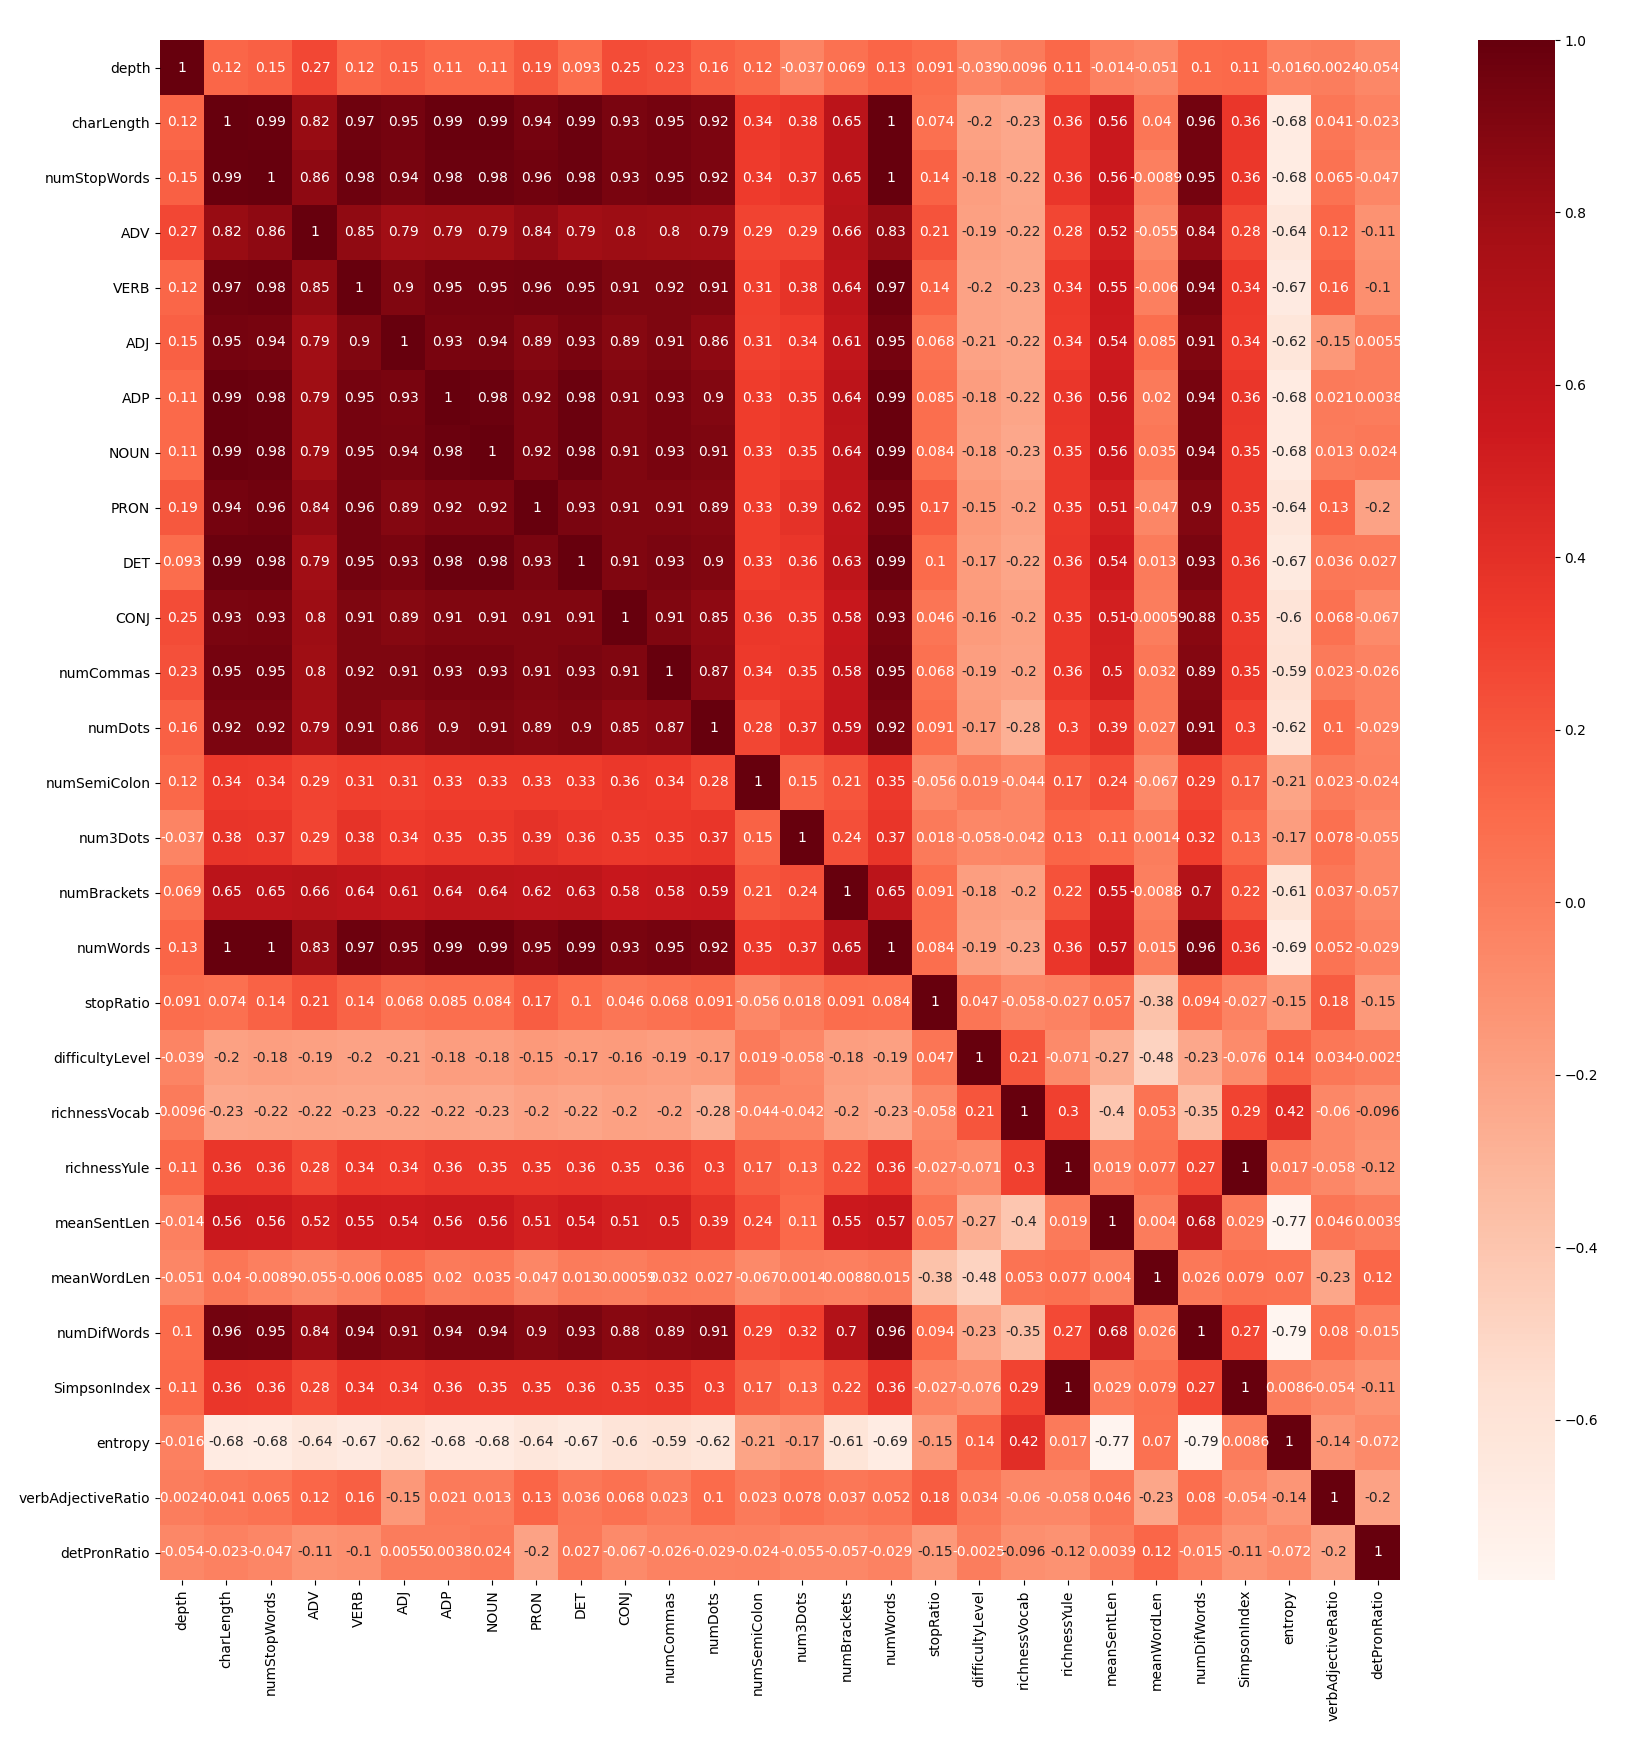
\includegraphics[width=0.98\paperwidth]{Imagenes/Bitmap/correlationmatrix.png}}%
	\caption{Pearson correlation coefficient between each pair of features}%
	\label{fig:correlation}
\end{figure}

In addition to the mentioned features, we have removed from our data set the following writing style markers: \textit{metricsSentences}, \textit{wordLength}, \textit{sentLength}, \textit{sentNumWords} and \textit{wordsAppearance}. All of them describe a distribution of a style feature (or several as the \textit{metricsSentence} attribute) through a dictionary or list structure, which are excessively complex to manipulate with the rest of the style features using common machine learning techniques. Furthermore, they would produce a big amount of NaN (Not a Number) values in our data set, because of the diversity in the number of sentences and words used in each e-mail (for instance if a message has an only sentence, all the style metrics related to the subsequent sentences will have a NaN value).

Therefore, we are going to work with 27 writing style markers, the depth of the message (perhaps we can find significant conclusions with this parameter) and the identifier of each message as index of each of the rows of our data set.

E-mail messages, by nature, do not contain a constant number of words from message to message. To overcome this variable and now that we have decided the style characteristics that we are going to study, the features are normalized, because techniques that require it (such as the K-Means algorithm) are used. Besides, we are going to find some NaN values, for example in \textit{verbAdjectiveRatio} and \textit{detPronRatio} in the messages that there are not adjectives or pronouns, respectively. The solution to overcome this problem, due to some algorithms do not admit data set with this type of values, is to assign the value of the arithmetic mean in the sample of individuals in the category to which the message belongs of the style marker in question, when it will be necessary. In other words, if an e-mail of the category $C$ has a NaN value in the style metric $M$, it will be replaced by the value of the arithmetic mean of the feature $M$ of the rest of the messages of class $C$.

It would be desirable to be able to visualize the main descriptive statistics to get an idea of each of the metrics. Nevertheless, given the big amount of style markers, the visualization becomes very complicated. For this reason, in this chapter, we are going to try to reduce the dimensionality of the system in order to be able to explain the main characteristics and describe the writing style.

Before starting with the data analysis, we are going to study the relationship between each selected feature. To carry out it, the Pearson correlation coefficient \citep{benesty2009pearson} is going to be calculated between each pair of style markers. It is a measure of linear dependence between two quantitative random variables. Unlike covariance, Pearson's correlation is independent of the scale of measurement of the variables. Less formally, we can define Pearson's correlation coefficient as an index that can be used to measure the degree of relationship of two variables as long as both are quantitative and continuous. It has a value between $-1$ and $+1$, where 1 is total positive linear correlation, $0$ is no linear correlation, and $-1$ is total negative linear correlation.

As a result of the calculation of the Pearson correlation coefficient, we obtain the heat map of the Figure \ref{fig:correlation}. Logically, there is a positive linear correlation between those metrics that are strongly influenced by the length of the message. These pairs of style markers represent almost all results obtained close to the value 1. Moreover, there is a total positive linear correlation between Yule's Characteristic and Simpson's Index, which was predictable given the definition of one style feature with respect to the other (see Section \ref{ssect:vocabf}). These relationship will be taken into account during the analysis of the data.